\section{Introduction of Ontologies into Ferda} \label{OntologiesFerda}

In this section we present the different functionalities and aspects of ontology management and exploitation as they have been implemented in Ferda.

\subsection{Ontology Representation Language Choice}

From the various possibilities we chose \emph{OWL} (Web Ontology Language, version 1.1) to represent ontologies, especially because it is a standard of W3C and it is widely supported by developers. 
As interface for manipulating with ontologies we used the Java OWL API parser\footnote{%
%Part of the CO-ODE project \url{http://co-ode.org}, 
Downloadable from \url{http://owlapi.sourceforge.net/}.}. 
The ontology was made accessible by a Ice middleware module in Ferda, which loads a local or remote OWL ontology and makes the content accessible for other modules of the Ferda system. 

\subsection{Mapping Ontologies to Database}

When binding a particular data source to a particular domain ontology, a mapping is to be established that connects individual data columns to entities from the ontology.
%one encounters problem of different naming of ontology and database. 
%The next step for usage of ontology was to construct mapping between ontology concepts and columns of the database. 
In Ferda we implemented a \emph{setting module} for manual mapping from data columns to ontology concepts. 
This mapping can be loaded and stored in an XML format, and thus can be created only once and then reused repeatedly. 
Figure \ref{fig:Mapping} shows the setting module that handles the mapping.

\begin{figure}[ht]
\centering
\mbox{\resizebox{120mm}{!}{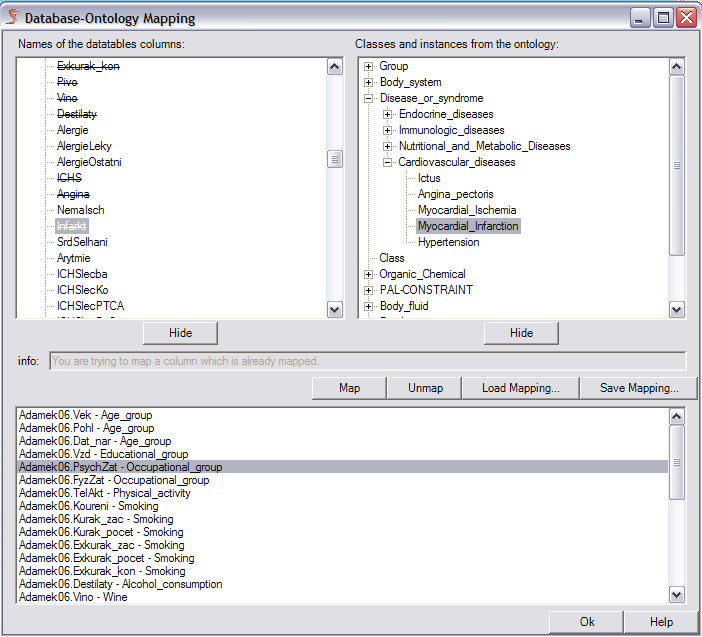
\includegraphics{Mapping.png}}}
\caption{Mapping database columns to ontology entities}
\label{fig:Mapping}
\end{figure}

Depending on the structure of the (OWL) ontology, the most adequate entity on which a data column should be mapped could be a concept, an instance, an object property, or, possibly most adequately from the formal point of view, a datatype property.
In the current version of Ferda, the user can map a data column to an ontology class or instance only: this is motivated by the experience that a \emph{class-centric} view is much more convenient to the user (when specifying the mappings) than a \emph{property-centric} view. 
We also do not allow mapping of one column to multiple classes or instances. 
%After conducting initial experiments with existing ontologies and databases, we allowed 
It is however possible to map multiple columns to one class or instance of the ontology. 
This situation occurs when the granularity of the data source is higher than the granularity of the ontology.
% (which is often the case). 

Each user can create his/her own mapping, but it is desirable to share a common mapping created by the domain expert. 
When the database is connected to the ontology via a mapping, Ferda automatically recognizes names of concepts from the ontology and uses them besides/instead of names from the database. 

\subsection{Storing Additional Information to Ontology}

As we mentioned in section \ref{OntologiesAssociation}, we need to store additional information in ontologies to enhance their usability for KDD. %Implementation from \cite{Zeman} attaches additional info to ontology classes. During later discussions with ontology specialists there was identified another approach for storing additional info. The main idea of is that additional info should not be attached to ontology classes, but to concrete ontology instances. This approach is more correct from the view of ontology design but is little bit less general than the first one. The second approach is a theoretical problem and there are none technical difficulties to update Ferda to be in accordance with it. The question is if it is really an advantage for end users.
In order to stay within the formalism of OWL, we use a \emph{meta-modelling} approach:
%Technical solution of enabling additional info saving is easy. 
for each type of additional information to be stored (such as attribute cardinality or important values dividing the domain) we created a special datatype property and set its domain to an OWL metaclass; currently we only use \emph{owl:Class} for simplicity. 
Thereafter, all classes can be equipped with this additional information type. 
%The reason why it is done through meta class is because we need to assign a concrete value to a information type. But if we would assign a slot to a class we would be able to assign value only to an instance what was not what we had wanted. With the new approach to information saving, this would be OK but it has one great disadvantage. You have to create one slot for each class where you want to save the additional information. So you would have to create N slots (where N is a count of classes) while in our implementation you can create it just once for all the classes. 

Information useful for data mining could alternatively be assigned to (especially, datatype) properties rather than to classes.
For this, it would suffice to connect the respective property to \emph{owl:DatatypeProperty} rather than to \emph{owl:Class}.
We are observing the development of the new version of the OWL standard, \emph{OWL~2} \cite{OWL2}, where some meta-modelling issues are handled in a novel way.

It is important to note that including such additional information into the ontology is not merely a matter of shifting the categorisation task from the data preparation phase to some previous phase.
Namely, the additional information items mentioned
\begin{itemize}
	\item are an inherent part of the \emph{domain}, and thus also deserve to be part of a domain ontology
	\item thanks to the persistence and potential web-based accessibility of the ontology, they can be repeatedly \emph{reused} by different people at different places
	\item their use is \emph{not restricted to data mining}, but they can also be exploited in other data-intensive ontology-driven tasks, such as in information extraction from text\footnote{The so-called extraction ontologies \cite{Embley,Prickl} share a lot with our approach mentioned.} or in data integration via ontology matching.
\end{itemize}

\begin{figure}[ht]
\centering
\mbox{\resizebox{120mm}{!}{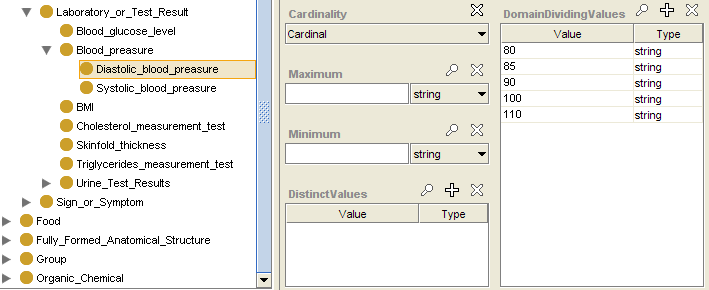
\includegraphics{Protege.png}}}
\caption{Including additional information in the ontology}
\label{fig:Protege}
\end{figure}

\subsection{Categorization of Attribute}
One of the main contributions of the ontology-based approach to the data preparation step is the ability to construct the attribute categorization automatically. 
In Ferda, \emph{attribute} boxes provide attribute categorization. 
Before the ontology support was implemented, the user could only use categorization algorithms to create equidistant or equifrequency intervals, or to create the categorization manually. 
This task was time consuming and had to be done over again. 
With ontological support, the user can create an \emph{ontology-derived attribute} box. 
This box loads information from the ontology and performs categorization based on additional information stored in the ontology. 
Figure~\ref{fig:Systolic} shows a histogram of the ontology-derived attribute \emph{systolic blood pressure} corresponding to the WHO guidelines for management of hypertension \cite{Hypertension}. 

\begin{figure}[ht]
\centering
\mbox{\resizebox{90mm}{!}{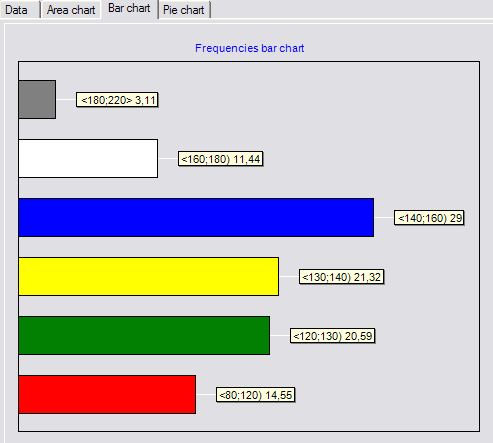
\includegraphics{Histogram.png}}}
\caption{Systolic blood pressure categories}
\label{fig:Systolic}
\end{figure}

\subsection{Identification and Exploitation of Semantically Related Attributes} \label{RelatedAttributes}
As was mentioned in section \ref{OntologiesDataPrep}, identification and usage of mutually related attributes helps the user in both the data preparation and task design stages of the data mining cycle. 
We used the \emph{box recommendation} mechanism, and offered the user semantic support (mainly at the level of naming and taxonomy) based on the ontology, as can be seen in Figure~\ref{fig:BoxesAsking}. 
When the user clicks on one item in the context menu, all data attributes corresponding to the entity from the ontology are created and added to the matrix for data mining.
For example, for the concept of \emph{Cardiovascular diseases}, attributes for individual findings such as \emph{Angina pectoris} or \emph{Myocardial ischemia} are added.

\begin{figure}[ht]
\centering
\mbox{\resizebox{110mm}{!}{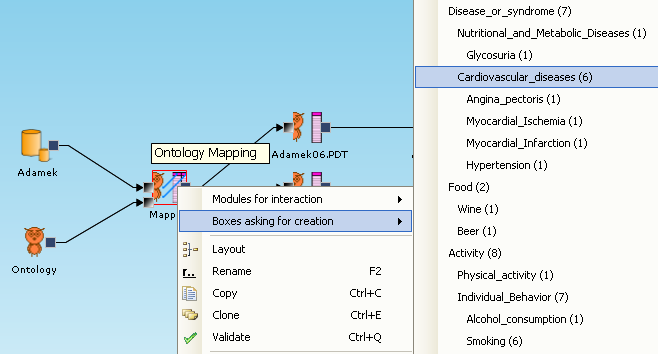
\includegraphics{BoxesAsking.png}}}
\caption{Semantics of attributes from the database}
\label{fig:BoxesAsking}
\end{figure}